\documentclass[a4paper, 10pt]{article}

%\usepackage{scalefnt}
%\usepackage{parcolumns}

\usepackage{newclude}
% Zum Einbinden in die Zusammenfassungs-files

\usepackage{amsmath,amsthm,amsfonts,amssymb} % Verbesserter Mathesatz
\usepackage{algorithm2e}
\usepackage{bigfoot} % komplexe Fußnotenapparate(Fußnoten in Fußnoten und andere Späße)%
\usepackage{colortbl}
\usepackage[T1]{fontenc} % normaler erweitere Zeichnesatz
\usepackage{framed, color}  % Ramenpaket für zum Einfügen von schönen Ramen
\usepackage{graphicx}
\usepackage{hyperref} %used for link to creative commons license
\usepackage{listings} %for code-listings (inkl. Tab-Styling)
\usepackage{marvosym}
\usepackage{marginnote}
\usepackage{microtype} % div. Verbesserungen des Schriftsatzes (Grauwert, opt. Randausgleich, Zeilenumbruch)
%\usepackage{multirow}
\usepackage{multicol} %use this with next line for vertical divided environment
%\setlength\columnseprule{.4pt}:465
\usepackage[ngerman]{babel} % Neue Rechtschreibung
\usepackage{pifont}
\usepackage[sans]{dsfont} %für alternative Mengensymbole
\usepackage{stmaryrd} %u.a. für \lightning
\usepackage{tikz} % für Diagramme(Dia!) und Bilder (z.B. *.eps)/für ER-Diagramme/für UML-Diagramme
%\usepackage{tikz-er2} %  er-diagramme
\usepackage{tikz-uml} % uml-Diagramme
\usepackage{units} % z.B. fuer \nicefrac{}{}
\usepackage[utf8]{inputenc} % utf8 für den Editor
\usepackage{wasysym} %u.a. für \lightning
\usepackage{xcolor}


\usetikzlibrary{shapes,decorations,arrows,fit,backgrounds} %Zum diversen zeichen%
%\usetikzlibrary{automata} % für den CFlipper, wenn es den soweit ist			%
\usetikzlibrary{positioning} % positionierung
%\usetikzlibrary{shadows} % fuer schoene schlagschatten
\usetikzlibrary{automata} % für Automaten

%%%%%%%%%%%%%%%%%%%%%%%%%%%
%  Formatierung der Seite
%%%%%%%%%%%%%%%%%%%%%%%%%%%
\usepackage{fancyhdr}
\pagestyle{fancy}		% für den footer										%
\renewcommand{\headrulewidth}{0pt} % damit oben kein dummer Strich kommt		%
\fancyhead{}
\topmargin -2cm 		% Oberer Rand											%
\textheight 25cm		% Texthöhe												%
\textwidth 16.0 cm		% Textbreite											%
\oddsidemargin -0.1cm 	% Warum?												%
\newcommand{\Gruppe}[2]
{
	\lfoot{#1}
	\rfoot{#2}
}
\colorlet{shadecolor}{gray!25} % Farbe für graue Box definieren
%%%%%%%%%%%%%%%%%%%%%%%%%%%%%%%%%%%%%%%%%%%%%%%%%%%%%%%%%%%%%%%%%%%%%%%%%%%%%%%%%
%Farben die definiert werden zum schreiben und zeichnen							%
%%%%%%%%%%%%%%%%%%%%%%%%%%%%%%%%%%%%%%%%%%%%%%%%%%%%%%%%%%%%%%%%%%%%%%%%%%%%%%%%%
\xdefinecolor{schwarz}{HTML}{000000}
\xdefinecolor{dunkelGruen}{HTML}{007D00}
\xdefinecolor{dunkelBlau}{HTML}{0000A0}
\xdefinecolor{dunkelRot}{HTML}{A00000}
\xdefinecolor{dunkelGelb}{HTML}{FFAA00}
\xdefinecolor{hellesGelb}{HTML}{FFCC00}
\colorlet{dGreen}{dunkelGruen}
\colorlet{dBlue}{dunkelBlau}
\colorlet{dRed}{dunkelRot}
\colorlet{dYellow}{dunkelGelb}

%%%%%%%%%%%%%%%%%%%%%%%%%%%%%%%%%%%%%%%%%%%%%%%%%%
%Farbliche Ausgaben:
%Parameter #1: Text oder Mathematische formel...
%z.B. : \gruen{Hallo Welt Test!}
%%%%%%%%%%%%%%%%%%%%%%%%%%%%%%%%%%%%%%%%%%%%%%%%%%

\newcommand{\yellow}[1]{\textcolor{dYellow}{#1}}
\newcommand{\gray}[1]{\textcolor{gray}{#1}}
\newcommand{\red}[1]{\textcolor{red}{#1}}
\newcommand{\green}[1]{\textcolor{green}{#1}}
\newcommand{\blue}[1]{\textcolor{blue}{#1}}
\newcommand{\dGreen}[1]{\textcolor{dGreen}{#1}}
\newcommand{\dBlue}[1]{\textcolor{dBlue}{#1}}
\newcommand{\dRed}[1]{\textcolor{dRed}{#1}}

%%%%%%%%%%%%%%%%%%%%%%%%%%%%%%%%%%%%%%%%%%%%%%%%
%Konfiguration für das darstellen von Quelltext
%%%%%%%%%%%%%%%%%%%%%%%%%%%%%%%%%%%%%%%%%%%%%%%%
\lstset
{
	language=Java, % oder C++, Pascal, {[77]Fortran}, ...
	numbers=left, % Position der Zeilennummerierung
	firstnumber=auto, % Erste Zeilennummer
	basicstyle=\ttfamily, % Textgröße des Standardtexts
	keywordstyle=\ttfamily\color{dRot}, % Formattierung Schlüsselwörter
	commentstyle=\ttfamily\color{dGruen}, % Formattierung Kommentar
	stringstyle=\ttfamily\color{dBlau}, % Formattierung Strings
	numberstyle=\tiny, % Textgröße der Zeilennummern
	stepnumber=1, % Angezeigte Zeilennummern
	numbersep=5pt, % Abstand zw. Zeilennummern und Code
	aboveskip=15pt, % Abstand oberhalb des Codes
	belowskip=11pt, % Abstand unterhalb des Codes
	captionpos=b, % Position der Überschrift
	xleftmargin=10pt, % Linke Einrückung
	frame=single, % Rahmentyp
	breaklines=true, % Umbruch langer Zeilen
	showstringspaces=false, % Spezielles Zeichen für Leerzeichen
	tabsize=2,
	texcl=true
}

%%%%%%%%
% Kopf
%%%%%%%%
\newcommand{\Header}[3]
{
	{\footnotesize \parindent0em
		{\sc Universität Konstanz}                \hfill #1 \\
		{\sc Fachbereich Informatik \& Informationswissenschaft} \hfill #2 \\
		#3 \hfill \today
	}
}

%%%%%%%%%%%%%%%%%%%%%%%
% load some java code
% \loadJava{file}
%%%%%%%%%%%%%%%%%%%%%%%
\newcommand{\loadJava}[1]
{
	\lstinputlisting[language=Java]{#1.java}
}

%%%%%%%%%%%%%%%%%%%%%%%
% load some cpp code
% \loadCpp{file.cpp}
%%%%%%%%%%%%%%%%%%%%%%%
\newcommand{\loadCpp}[1]
{
	\lstinputlisting[language=C++]{#1}
}

%%%%%%%%%%%%%%%%%%%%%%%%%%%%%
% load some code
% \loadCode{Python}{file.py}
%%%%%%%%%%%%%%%%%%%%%%%%%%%%%
\newcommand{\loadCode}[2]
{
	\lstinputlisting[language=#1]{#2}
}

%%%%%%%%%%%%%%%%%%%%%%%%%%%%%%%%%%%%%%%%%%%%%%%%%%%%%%%%%%%%%%%%%%%%%%%
% some symbols
%%%%%%%%%%%%%%%%%%%%%%%%%%%%%%%%%%%%%%%%%%%%%%%%%%%%%%%%%%%%%%%%%%%%%%%
\newcommand{\correct}{\green{\text{\ding{52}}}} %for use in text and math
\newcommand{\wrong}{\red{\text{\ding{56}}}} %for use in text
\newcommand{\tflash}{$\yellow{\lightning}$} %for use in text
\newcommand{\mflash}{\yellow{\lightning}} %for use in math
\newcommand{\follows}{$\Rightarrow$} %used so often...
\newcommand{\good}{\item[\dGreen{\ding{58}}]} %an item with a green plus as bullet point
\newcommand{\bad}{\item[\red{\Emailct}]} %better icon for bad items
\newcommand{\note}[1]{\red{\marginnote{#1}}} %add a red margin note
\newcommand{\fitem}{\item[\follows]} %items with a follows arrow
\newcommand{\hm}{\ensuremath{\overset{-\mkern-11mu-\mkern-3.5mu\rhook}{\smash{\odot}\rule{0ex}{.46ex}}\underline{\hspace{0.5em}}\overset{-\mkern-11mu-\mkern-3.5mu\rhook}{\smash{\odot}\rule{0ex}{.46ex}}}}

%%%%%% make emph bold instead of italic %%%%%
\makeatletter
\DeclareRobustCommand{\em}{%
  \@nomath\em \if b\expandafter\@car\f@series\@nil
  \normalfont \else \bfseries \fi}
\makeatother

%%%%%%%%%%%%%%%%%%%%%%%%%%%%%%%%%%%%%%
% languages for \loadCode
%ABAP		IDL				Plasm
%ACSL		inform			POV
%Ada		Java			Prolog
%Algol		JVMIS			Promela
%Ant		ksh				Python
%Assembler	Lisp			R
%Awk		Logo			Reduce
%bash		make			Rexx
%Basic		Mathematica1	RSL
%C			Matlab			Ruby
%C++		Mercury			S
%Caml		MetaPost		SAS
%Clean		Miranda			Scilab
%Cobol		Mizar			sh
%Comal		ML				SHELXL
%csh		Modula-2		Simula
%Delphi		MuPAD			SQL
%Eiffel		NASTRAN			tcl
%Elan		Oberon-2		TeX
%erlang		OCL				VBScript
%Euphoria	Octave			Verilog
%Fortran	Oz				VHDL
%GCL		Pascal			VRML
%Gnuplot	Perl			XML
%Haskell	PHP				XSLT
%HTML		PL/I
%%%%%%%%%%%%%%%%%%%%%%%%%%%%%%%%%%%%%%

\usetikzlibrary{trees}

\begin{document}

\Gruppe{Stephan Heidinger}{SEng - Zusammenfassung v0.1}
\Header{Software Engineering}{Wintersemester 2011/2012}{Stephan Heidinger}

\begin{shaded}
Dieses Dokument wurde unter der Creative Commons - Namensnennung-NichtKommerziell-Weitergabe unter gleichen Bedingungen (\textbf{CC by-nc-sa}) veröffentlicht. Die Bedingungen finden sich unter \href{http://creativecommons.org/licenses/by-nc-sa/3.0/de}{diesem Link}. \\
\centerline{
\includegraphics[scale=1]{../cc-by-nc-sa.png} }
\end{shaded}

\textit{Find any errors? Please send them back, I want to keep them!}

\begin{shaded}
\textbf{Definitions for Software Engineering} \\
``Multi-person construction of multi-version software'' (D. Parnas, 1987)\\
``The application of a systematic, disciplined, quantifiable approach to the development, operation, and maintenance of software; that is, the application of engineering to software.''
\end{shaded}

\tableofcontents
\newpage

\section{Software Crisis}
Term from NATO study group in 1967.
\begin{description}
	\item[fault] mistake/error made by a human during a software activity (erroneous design, requirements, coding)
	\item[failure] observed departure of a system from the desired state
\end{description}
\subsection{symptoms}
\begin{itemize}
	\item products are delivered late \follows high cost
	\item projects exceed budgeds \follows high cost \follows waste of resources
	\item product doesn't do, whats its supposed to do \follows inefficient \follows hight cost
	\item products are defective \follows high cost (failures, maintenance,\dots), ethical considerations
	\item projects get abandonded before delivery \follows waste of resources
\end{itemize}

\subsection{Characteristics of software}
\begin{itemize}
	\item Software is \emph{engineered}, not manufactured (custom built, little to no (mechanical) assembly, human intensive process)
	\item Software does not wear out (but: change of requirements, changes in environment)
	\item software is \emph{complex}
	\item software is \emph{detemining system factor} (up to 80\% of development effort)
\end{itemize}

\subsection{Why is software difficult to produce?}
\begin{itemize}
	\item no similiar system built so far (problems unknown, assumptions about environment may be wrong)
	\item \emph{Requirements} are not well understood/phrased
	\item Requirements \emph{change} during development
	\item complex \emph{interaction}
	\item nature of systems:
		\begin{itemize}
			\item concurrent systems (races, deadlocks, \dots)
			\item embedded systems (hardware interaction, timing, \dots)
			\item information systems (complexity, legacy, \dots)
		\end{itemize}
	\item software is \emph{easily changeble} \follows ``code and fix''
	\item software is \emph{discreet} (either fails, or doesn't)\marginnote{Stimmt auch nicht immer\dots}
\end{itemize}

\subsection{Software Debvelopment Myths}
\begin{itemize}
	\item Management
		\begin{itemize}
			\item standard books, software, tools, \dots \follows software hard to standardize
			\item behind schedule? add programmers! \follows effort to integrate new people
		\end{itemize}
	\item Customer
		\begin{itemize}
			\item general statement of objectives sufficient
			\item change (as in requirements) can easily be implemented
		\end{itemize}
	\item Pracitioner
		\begin{itemize}
			\item once programm is running, job is done
			\item until programm is running, no way to check quality
			\item only deliverable is working programm
		\end{itemize}
\end{itemize}

\subsection{Software Engineering}
Communication between a huge number of parties (customer, end user, sw designer, developer, \dots) must be maintained. \\
Highly complex systems: SE has to provide solutions.

\begin{description}
	\item[\follows] base sw production on engineering approach
	\item[\follows] design sw as a \emph{process} that supports
		\begin{itemize}
			\item correctness \& dependability
			\item cost-effectivenes
			\item complexity of project
			\item longevity of product, life cycle, changes
			\item communication amongst parties
		\end{itemize}
	\item[\follows] software engineering process model
\end{description}

\section{waterfall model}
\begin{tikzpicture}[node distance=50]

\node[draw] (1) at (0,0) {System Design};
\node[draw] (2) [below right of = 1] {Requirements};
\node[draw] (3) [below right of = 2] {Design};
\node[draw] (4) [below right of = 3] {Implementation};
\node[draw] (5) [below right of = 4] {Integration};
\node[draw] (6) [below right of = 5] {Maintenance};

\node (c1) [right of = 1] {};
\node (c2) [right of = 2] {};
\node (c3) [right of = 3] {};
\node (c4) [right of = 4] {};
\node (c5) [right of = 5] {};
\node (c6) [right of = 6] {};

\node (1c) [left of = 1] {};
\node (2c) [left of = 2] {};
\node (3c) [left of = 3] {};
\node (4c) [left of = 4] {};
\node (5c) [left of = 5] {};
\node (6c) [left of = 6] {};

\path[draw,->] (1) .. controls (c1) .. (2);
\path[draw,->] (2) .. controls (c2) .. (3);
\path[draw,->] (3) .. controls (c3) .. (4);
\path[draw,->] (4) .. controls (c4) .. (5);
\path[draw,->] (5) .. controls (c5) .. (6);

\node[node distance=10] (a1) [right of = c1] {};
\node[node distance=10] (a2) [right of = c2] {\textsc{Srs}};
\node[node distance=10] (a3) [right of = c3] {Design};
\node[node distance=10] (a4) [right of = c4] {\textcolor{gray}{Test}};
\node[node distance=10] (a5) [right of = c5] {\textcolor{gray}{Test}};
\node[node distance=10] (a6) [right of = c6] {};

\path[draw,dashed,color=gray,->] (2) .. controls (2c) .. (1);
\path[draw,dashed,color=gray,->] (3) .. controls (3c) .. (2);
\path[draw,dashed,color=gray,->] (4) .. controls (4c) .. (3);
\path[draw,dashed,color=gray,->] (5) .. controls (5c) .. (4);
\path[draw,dashed,color=gray,->] (6) .. controls (6c) .. (5);

\node[node distance=20] (1a) [left of = 1c] {};
\node[node distance=20] (2a) [left of = 2c] {\textcolor{red}{``what''}};
\node[node distance=20] (3a) [left of = 3c] {\textcolor{red}{``how''}};
\node[node distance=20] (4a) [left of = 4c] {};
\node[node distance=20] (5a) [left of = 5c] {};
\node[node distance=20] (6a) [left of = 6c] {};

\end{tikzpicture}

\begin{description}
	\item[System Design] problem \& System requirements, fesability study, define main subsystems (allocate to hw/sw), system design document (\textsc{Sdd}, informal, with customer, somtimes: user manuals, user interfaces, test plans)
	\item[Requirements] requirement analysis (``what'' the system has to do (not how), software requirements describing observable external behaviour (functional, nonfunctional)), software requirement specification (\textsc{Srs})
	\item[Design] ``how'' the system is working, architectural (high level) design (decompose problem into components, global data structures, internal interfaces), detailed design (algorithmic design, internal data structures, programming language(s))
	\item[Implementation] (and Testing) \follows translate design modules into code, test modules in isolation
	\item[Integration] (and Testing) integrate tested modules to form system, \emph{integration testing}, validation, customer accptance tests
	\item[maintenance] deploy product, perform maintenance (corrective, adaptive, perfective), retire product
\end{description}
\subsubsection{Benefits}
\begin{itemize}
	\item Definition of seperate Tasks (Seperation of concerns)\\dividing complex design problems into smaller units \follows facilitates team work/reproducibility
	\item specification and documentation  \follows enforces documentation, facilitates testing (against requirements specification)
	\item further concepts
		\begin{itemize}
			\item verification / validation (compare intermediate results with requirements and design)
			\item prototyping (mock-up available early, reduces risk)
			\item evolutionary process model (accommodate change)
		\end{itemize}
\end{itemize}

\subsubsection{Defects}
\begin{itemize}
	\item no feedback loops
	\item document driven, inflexible
	\item large time gap between inception and completion
\end{itemize}

\subsubsection{Alternatives}
\begin{itemize}
	\item modified waterfall model
	\item V-Model, V-Model XT
	\item Evolutionary Process models
	\item Spiral model
	\item Rational Unified Process
	\item Agile Processes
	\item \dots
\end{itemize}

\subsection{Software Qualities}
\begin{description}
	\item[Correctness:] the software behaves according to the \emph{requirement specification}
	\item[Reliability:] the software guarantees a level of quality service ($<$Correctness)
	\item[Robustness:] the software behaves ``reasonably'' even in unexprected circumstances (e.g. input, power failure, \dots)
	\item[Maintainability:] software is easy to maintain/extend
	\item[Performance:] system is usable (e.g. input response)
	\item[Reusability:] re-use of previously used, tested and verified code
	\item[Interoperability:] standardisation, interfaces, \dots
\end{description}

\subsection{Software Engineering Principles}
\begin{description}
	\item[Rigor:] use a method and apply it rigorously to every step
	\item[Formality:] use (mathematical) formalizable methods and notations
	\item[Speration of Concerns:] deal with different aspects in seperate steps
	\item[Abstraction:] seperate the concern of the important aspects from the concern of unimportant ones
	\item[Modularity:] decompose problem into independent modules \follows separation of concern
	\item[Generality:] focus on the discovery of more general problems
\end{description}

\section{Requiremnt \& Analysis}

\subsection{Requirement Elicitation}
\begin{shaded}
``A \textbf{requirement} is a condition or capability that must be met or professed by a system component to satisfy a contract, standard, specification or other formally inposed document.'' \\
(ANSI/IEEE Standard 729-1983)
\end{shaded}
requirements \follows description of the \emph{externally visible (interface) \marginnote{not environment behaviour}behaviour}, the ``what''\\
Interaction between the system and the system-relevant portion of the envrionment

\begin{description}
	\item[User (Client) requirements:] statements in natural language plus diagramms
	\item[System requirements:] structured document, detailed description of system's functions, services and operational constraints; may be part of contract between client and contractor
\end{description}
\subsubsection{Types of requirements}
\begin{description}
	\item[functional requirements:] high-level-``what'' the system should do
		\begin{itemize}
			\item statement which services the system should provide
			\item interaction between system and environment (system states, i/o)
			\item how the system should behave in particular situations
			\item describe the system services in detail
			\item often included with ``shall/should''
		\end{itemize}
	\item[nonfunctional requirements:] (if not met, system may be useless (not usable)) \\
	nonfunctional requirements often have quantitative measures (MB, training time, availability, \dots)\\
	\begin{tikzpicture}[
	dist0/.style={},
	dist1/.style={sibling distance=11em},
	dist2s/.style={sibling distance=5.2em},
	dist2b/.style={sibling distance=6.4em},
	down/.style={level distance=7ex},
	downB/.style={level distance=20ex},
	level0/.style={draw,rectangle,fill=blue!20,rounded corners=.8ex},
	level1/.style={draw,rectangle,fill=green!20,rounded corners=.8ex},
	level2/.style={draw,rectangle,fill=yellow!20,rounded corners=.8ex},
	level3/.style={draw,rectangle,fill=gray!20,rounded corners=.8ex},
]

	\coordinate
	child[grow=down,anchor=south, level distance=0ex] {node[level0] {non-functional}}
	[edge from parent fork down]
		child[dist1,down] {node[level1] {product}
			child[dist2s,down] {node[level2] {usability}
			}
			child[dist2s,down] {node[level2] {efficiency}
				child[dist2s,down] {node[level3] {performance}}
				child[dist2s,down] {node[level3] {space}}
			}
			child[dist2s,down] {node[level2] {reliability}
			}
			child[dist2s,down] {node[level2] {portability}
			}
		}
		child[dist1,down] {node[level1] {organisational}
			child[dist2b,downB] {node[level2] {delivery}
			}
			child[dist2b,downB] {node[level2] {implementation}
			}
			child[dist2b,downB] {node[level2] {standards}
			}
		}
		child[dist1,down] {node[level1] {external}
			child[dist2b,down] {node[level2] {interoperability}
			}
			child[dist2s,down] {node[level2] {ethical}
			}
			child[dist2s,down] {node[level2] {legislative}
				child[dist2s,down] {node[level3] {privacy}}
				child[dist2s,down] {node[level3] {safety}}
			}
		}
;
\end{tikzpicture}
		\begin{itemize}
			\item not primarly related to sytem's funcions/services, but to quality and additinal (quantitative) characteristics
			\item constraints on the services/functions:
			\begin{itemize}
				\item reliability (avalability, integrity, security, safety)
				\item accuracy of results
				\item performance / timing
				\item human-computer interface issues
				\item operating and physical constraints
				\item portability and interoperatbility
				\item reliability
				\item response time
				\item storage requirements
				\item standards \dots
				\item also: particular system, programming language or development method
			\end{itemize}
			\item product requirements (product must behave in particular way (execution time, speed, reliability, \dots))
			\item organisational requirements (standards used, impelementation requirements, \dots)
			\item external requirements (interoperatbility/legislative requirements, \dots)
		\end{itemize}
		\item[domain requirements:] (if not met, system may be unworkable in that domain)
			\begin{itemize}
				\item derived from application domain
				\item characteristics/features of domain
				\item constraints on existing requirements
				\item define specific computations
				\item may be expressed in domain specific language \follows often hard to understand
				\item often implicit \follows hard to aquire
			\end{itemize}
\end{description}


\subsubsection{Requirement Specification Properties}
\begin{description}
	\item[correctness:] facts in requirement specification \follows required properties of the system
	\item[unambiguity:] all specifications have a single interpretation
	\item[completeness:] 
		\begin{enumerate}
			\item every property required of the system is expressed in the specification\\
			{\small does this include things that are \emph{not permitted?}}
			\item the responses of the software system on all types of possible input values are specified
			\item \dots {\small (more possible)}
		\end{enumerate}
	\item[verifiability:] there exists an effective (manual/automatic) process for checking wether a software product satisfies the required properties (formal verification (mathematical proof) or validation (model checking, testing, simulation)), often not possible for every requirement
	\item[consistency:] no two requirements contradict each other: never $A \wedge \neg A$
	\item[traced:] origin of every requirement is clear
	\item[traceable:] requirement specification is edited so it is easy to reference every single requirement (e.g. numbering)
	\item[design independent:] the requirement specification does not require specific software/architecture/algorithms
\end{description}

\subsubsection{Activities during the requirement Stage}
	\begin{description}
		\item[starting point] 
			\begin{itemize}
				\item customer requirements (abstract)
				\item system specification document (hw \& sw)
			\end{itemize}
		\item[Activities (Kotonya+Sommerville)]
			\begin{itemize}
				\item requirement elicitation\marginnote{Elicitation \follows Herausholen} (interviews, scenarios, market observation, \dots) \\
				determine, which of possibly contradictory requirements are important
				\item requirement documentation and specification (comprehensible requirements document)
				\item requirement validation (consistency, completeness, correspondence of documented requirements and abstract customer or user requirements)
			\end{itemize}
			\begin{tikzpicture}[%
	>=stealth,
	node distance=3.5cm,
	on grid,
	auto,
	io/.style={draw, text width=2.5cm, align=center},
	proc/.style={draw, rounded corners=1.2em, text width=2.5cm, align=center},
	dist/.style={node distance = 3cm},
	dick0/.style={draw,line width=1.5pt},
	dick/.style={dick0,->},
	duenn/.style={draw,line width=1.5pt,dashed,->}
]

\node[io] (root) at (0,0) {customer or user requirements (abstract)};

\node[proc] (2) [below left of  = root] {requirements analysis and negotiation};
\node[proc] (1) [left of       = 2   ] {requirements elicitation};
\node[proc] (3) [below right of = root] {requirements documentation and specification};
\node[proc] (4) [right of      = 3   ] {requirements validation};

\node[io,node distance=2cm] (leaf) [below of = 3] {negotiated and validated requirements};

\node[node distance=1.5cm] (phantom1) [below left of =root] {};
\node[node distance=1.5cm] (phantom2) [below right of =root] {};

\path[dick] (root) -| (1);
\path[dick] (1) -- (2);
\path[dick] (2) -- (3);
\path[dick] (3) -- (4);
\path[dick] (3) -- (leaf);
\path[duenn] (root) -| (4);

\path[dick] (phantom2) -| (1.north east);
\path[dick] (phantom2) -| (2);
\path[dick] (phantom1) -| (3);
\path[dick0] (phantom1) -| (4.north west);


%	\node[state] (A)              {A};
%	\node        (B) [right of=A,fill=blue!25,text width=3cm]{This is a demonstration text for showing how line breaking works.};;
%	\path[->] (A) edge (B);


\end{tikzpicture}
			\item[social activity:]
			Not a single person knows everything about the system \follows communication is needed \follows difficult (technical language, ambiguities, customers not aware of needs, personalities.)
	\end{description}

\subsubsection{Interviewing / Structured Questioning Techniques}
\begin{enumerate}
	\item context-of-system (why are we building this system/who are the users/critical functionality/needs)
	\item open-ended questions (produce large amount of info/use, when not much known yet
	\item close-ended questions (specific questions))
	\item rephrase questions (make sure answers understood right/inconsistencies/ambiguities)
	\item whom else to interview
\end{enumerate}

\subsubsection{Learning from Existing Systems}
\begin{itemize}
	\item analyse user manuals
	\item use/play with existing systems
	\item market analysis (competing systems, market research, which features to be included
	\item reverse engineering)
\end{itemize}

\subsubsection{requirement uncertainty}
When the customer does not know, what he really needs/wants \follows prototype.
Built prototype early (only if prototype build is faster than system build),
use prototype for requirement elicitation.
Prototyping also part of some life cycle and process models (spiral model)

\subsubsection{Requirements Gathering - Brainstorming}
\begin{itemize}
	\item generate ideas (free of criticism/judgement) \follows as many ideas as possible
	\item discuss, revise, organize ideas
	\item evaluate, prioritize
\end{itemize}

\subsubsection{\textsc{Fast} (Facilitated Application Specification Technique)}
\begin{itemize}
	\item overcome we/then attitude (developer/user/customer)
	\item team oriented
	\item guidelines:
		\begin{itemize}
			\item must participate entire meeting
			\item participants are queal
			\item preparation as important as meeting
			\item pre-meeting documents are only ``proposed''
			\item off-site location preferred
			\item set agenda, maintain ist
			\item no technical details
		\end{itemize}
\end{itemize}

\subsubsection{\textsc{Jad} (Joint Application Design, 1977)}
\begin{itemize}
	\item technique to get all participants to aggree on sw requirements and design
	\item 20\% reduction of life cylce cost, \~15\% functionality less missed
	\item \textsc{Jad}/Plan \follows software requirement elicitation
	\item \textsc[Jad]/Design \follows software design
	\item Main Objective:
		\begin{enumerate}
			\item group dynamics \follows enhace capcabilites ofindividuals
			\item communication and understanding \follows use of visual 	aids
			\item rational, organized process \follows repeatability
			\item standardized documentations \follows use of standard forms
		\end{enumerate}
	\item customisation (prepare tasks for session)
	\item session (customized, facilitated meetings (developers and user))
	\item wrap-up (finalize results from sesion)
	\item participants
		\begin{description}
			\item[session leader:] manages sessions, management/communications skills, problem domain competence
			\item[analyst:] \follows session output, technical understanding req.
			\item[executive sponsor:] high-level strategic insight into system, executive-level decissions (resources, \dots)
			\item[user representative:] ``user''
			\item[information systems representative:] feasibility assessment
			\item[specialist:] knowledge from application domain
		\end{description}
	\item Customization phase
	\begin{itemize}
		\item orientation (sponsor endorses project, session leaders (+analyst) gains understanding of system/environment)
		\item organize team (select participants, think of questions ahead)
		\item tailor the process (how much time/resources, customize documents)
		\item prepare materials (slides, presentations, \dots, white boards, flip chats, \dots, agenda)
	\end{itemize}
	\item Session phase
	\begin{itemize}
		\item orientation (welcome, overview)
		\item define high-level requirements (objectives, benefits, strategic/future considerations, constraints and assumptions, security/audit/control) \follows recorded by analyst, discussion (refine, assess requirements)
		\item defince scope of system (organize and prioritize requirements, scopes, s.t. system meets objectives, but not too costly or complex)
		\item prepare \textsc{Jad}/Design (estimate resources, identify participants, schedule meetings)
		\item document issues and considerations (problems that affect requirements \follows assign a person for resolution)
		\item conclusion (review information and decissions, voice remaining concerns, conclude s.t. particip. have sense of ownership/commitment)
	\end{itemize}
	\item Warp-Up Phase
	\begin{itemize}
		\item transform session documents into formal planning documents (analyst)
		\item edit \textsc{Jad}/Plan
		\item review \textsc{Jad}/Plan (all participants \follows changes possible
		\item sponsor approval)
	\end{itemize}
\end{itemize}

\subsection{Object Oriented Analysis}
mapping onto waterfall process
\begin{itemize}
	\item requirements \follows object-oriented \emph{analysis}
	\item architectural design \follows system design
	\item detailed design \follows object design
\end{itemize}
oo swe processes are \emph{more continuous}
\begin{itemize}
	\item which are \emph{objects of interest}
	\item what are they doing
	\item \textsc{Uml} use case, sequence, class diagrams
\end{itemize}

\begin{shaded}
\textbf{Object} \marginnote{J. Rumbaugh et al}\\
``A discrete entity with a well defined boundary and identity that encapsulates state and behaviour; ...'' \\
``A concept, abstraction or thing with crisp boundaries and meaning for the problem at hand...''\\
``Objects serve two purposes: The promote understanding of the real world and provide a practical basis for computer implementation'' \\
``All objects have identity and are distinguishable.''
\end{shaded}

\subsubsection{Obejct-Oriented Software Engineering}
\begin{itemize}
	\item software is defined with
	\begin{description}
		\item[objects:] entities, correspondence in real world (identity, attributes, methods)
		\item[classes:] abstact of objects
	\end{description}
	\item objects encapsulate data (interface to data)
	\item interface is relevant, not implementation
	\item reuse through inheritance
	\item abstraction through polymorphism
\end{itemize}

\subsubsection{Software Models}
\begin{itemize}
	\item software systems complex \follows break down into subproblems
	\item software models \follows abstraction of real world
	\item usage
		\begin{description}
			\item[eary life-cycle stages:] evaluate properties of real-world system (elicitate, document, verify, validate requirements, simulation)
			\item[design stage:] document architecture, assess performance/behaviour
			\item[implementation/coding stage:] automatically synthesize code (class skeletons, state machine behaviour)
			\item[testing stage] what to test (requirements models)
			\item[maintenance stage:] document existing system for evolution
		\end{description}
\end{itemize}

\subsection{Analysis with the UML}
\begin{itemize}
	\item visual notation for analysis and design
	\item standardized by \emph{Object Management Group} \url{http://www.omg.org}
\end{itemize}

\subsubsection{Static}
\begin{description}
	\item[Use Case Diagrams]
	\begin{itemize}
		\item often first step i OO-dev-process
		\item a use case represents a usage scenario (atomic)
		\item documents the functinoalities the system provides to user (``what'' does the system do)
		\item actors (anything or anyone interacting with the system, provide input/output) and principal use cases (interaction between actor and system)
		\item \begin{tikzpicture}[
]

\begin{umlsystem}[x=4, fill=red!10]{The system}
\umlusecase{use case1}
\umlusecase[y=-2]{use case2}
\umlusecase[y=-4]{use case3}
\umlusecase[x=4, y=-2,]{use case4}
\umlusecase[x=6, fill=green!20]{use case5}
\umlusecase[x=6, y=-4]{use case6}
\end{umlsystem} 

\umlactor{user}
\umlactor[y=-3]{subuser}
\umlactor[x=14, y=-1.5]{admin}

\umlinherit{subuser}{user}
\umlassoc{user}{usecase-1}
\umlassoc{subuser}{usecase-2}
\umlassoc{subuser}{usecase-3}
\umlassoc{admin}{usecase-5}
\umlassoc{admin}{usecase-6}
\umlinherit{usecase-2}{usecase-1}
\umlHVextend[name=extd]{usecase-4}{usecase-5}
\umlinclude[name=incl]{usecase-3}{usecase-4}

\umlnote[x=7, y=-6]{incl-1}{use case3 uses something of use case4}
\umlnote[x=7,y=2]{extd-1}{use case5 might lead to use case4}

\end{tikzpicture}
		\item <<include>> \follows a use case uses functionality from another use case
		\item <<extend>> \follows exceptional or optional behaviour
	\end{itemize}
	\item[Class Diagrams:]
	\begin{itemize}
		\item Phenomen (object in the world of a domain as perceived
		\item Concept (properties iof a phenomen) is a 3-tuple: name (distringuishes it from others), purpose (properties that determine, if phenomen is member of concept), members (phenomena, that are part of concept)
		\item Type (abstraction in context of programming (name: int) \\
		\texttt{SimpleWatch} or \texttt{Firefighter}
		\item Class (abstraction in the context of oo-languages, encapsulates state(variables) and behaviour(methods))
		\item Instance (existing instance of a class) \underline{\texttt{myWatch:SimpleWatch}} or \underline{\texttt{Joe:Firefighter}}
		\item \begin{tikzpicture}[]

\begin{umlpackage}{package}
\umlclass[template=T]{Template Class}{
  n : uint \\ t : float
}{}
\umlclass[x=4]{real class}{
  d : double
  }{
  \umlvirt{setB(b : B) : void} \\ getB() : B}
\end{umlpackage}


\end{tikzpicture}
		\item Generality (most general aspect of problem)
		\item Abstraction (not individual objects, what they have in common)
		\item 		``The descriptor for a set of objects that share the same attributes, relationships and behavior. A class represents a concept within the system being modeled.''
		\item used during requirement analysis (model problem domain concepts), system design (model subsystems and interfaces), object design (model prog language classes)
		\item Association: ``A semantic condition or restriction represented as an expression.'' \\
		\begin{tikzpicture}[]
\umlclass[x=-3,y=0]{Person}{name: String \\ age: Integer}{}
\umlclass[x=3,y=0]{Company}{name: String}{}
\umlassoc[mult1=0..*,mult2=*,name=contract]{Person}{Company}
\umlclass[x=0,y=2]{WorkContract}{salary: Integer}{terminate()}
\umlassoc[style=dashed]{WorkContract}{contract-1}

\umlclass[x=-3,y=-2.5]{Person}{name: String \\ age: Integer}{}
\umlclass[x=3,y=-2.5]{Car}{make: carMakers \\ color: carColors}{}
\umlassoc[mult1=1,mult2=0..*]{Person}{Car}

\umlclass[x=-3,y=-4.5]{Triangle}{}{}
\umlclass[x=3,y=-4.5]{Corners}{}{}
\umlassoc[mult1=1,mult2=3]{Triangle}{Corners}


\end{tikzpicture}
		\item Dependencies: \\
		\begin{tikzpicture}[]

\umlclass[x=-3,y=0]{BoxOffice}{}{}
\umlclass[x=3,y=0]{SchedulingEngine}{}{}
\umlimpl[stereo=use]{BoxOffice}{SchedulingEngine}

\end{tikzpicture}
		\item Aggregation: \\
		\begin{tikzpicture}[]
\umlclass[x=-0,y=0]{Document}{}{}
\umlclass[x=0,y=-3,name=Toc]{Table of Contents}{}{}
\umlclass[x=3,y=-3]{Section}{}{}
\umlclass[x=-3,y=-3]{Index}{}{}
\umlVHVaggreg[mult2=1,pos=2.5]{Document}{Index}
\umlaggreg[mult2=1..*]{Document}{Toc}
\umlVHVaggreg[mult2=0..1,pos=2.5]{Document}{Section}

\end{tikzpicture}
		\item Composition \\
		\begin{tikzpicture}[]
\umlclass[x=-0,y=0]{Company}{}{}

\umlclass[x=2,y=-3]{Departement}{}{}
\umlclass[x=-2,y=-3]{Office}{}{}
\umlVHVcompo[mult2=1..*,mult1=1,pos=2.5]{Company}{Departement}
\umlVHVcompo[mult2=1..*,pos=2.5]{Company}{Office}
\umlcompo[mult=*, angle1=0, angle2=-90, loopsize=2.5cm]{Departement}{Departement}

\end{tikzpicture}
		\item Generalisation \\
		\begin{tikzpicture}[]
\umlclass[x=-0,y=0]{Staff}{name: String\\SIN: Integer}{calc\_paycheck()}
\umlclass[x=2,y=-4]{SupportStaff}{hours: Integer \\ overtime: Integer \\ hourly\_rate: Integer}{calc\_paycheck()}
\umlclass[x=-2,y=-4]{Engineer}{clearance: Boolean\\salary: Integer}{calc\_paycheck()}
\umlVHVinherit[]{SupportStaff}{Staff}
\umlVHVinherit[]{Engineer}{Staff}

\end{tikzpicture}
		\item Visibility (+ public, - private, \# protected)
	\end{itemize}
\end{description}

\subsubsection{Dynamic}
\begin{description}
	\item[Sequence Diagrams] used during requirement analysis (refinde dynamic behaviour), design (document subsystem interfaces), good for real-time specifications\\
	\begin{tikzpicture}
\begin{umlseqdiag}
%\umlobject[class=simpleWatch,stereo=actor]{myWatch}
%\umlactor[class=simpleWatch]{myWatch}
%\umlentity[class=simpleWatch]{myWatch}
%\umlboundary[class=simpleWatch]{myWatch}
%\umlcontrol[class=simpleWatch]{myWatch}
%\umldatabase[class=simpleWatch]{myWatch}
%\umlmulti[class=simpleWatch]{myWatch}
%\umlobject[class=simpleWatch]{b}

\umlactor[class=WatchUser]{a}
\umlobject[class=SimpleWatch]{b}
\umlobject[class=SomethingElse]{c}

\begin{umlcall}[op={pressButton1()},type=synchron, return=0]{a}{b}

\end{umlcall}

\begin{umlcall}[op={doSomething()}]{a}{c}

\end{umlcall}

\end{umlseqdiag}
\end{tikzpicture}
	\begin{itemize}
		\item classes \follows columns
		\item messages \follows arrows
		\item return values  \follows dashed arrows
		\item activations \follows narrow rectangles
		\item lifelines \follows dashed lines
	\end{itemize}
	\item[State Chart Diagram] state machine description (only for dynamically interesting objects)
	\item[Dynamic Modeling:] Collection of State Chart Diagrams
\end{description}

Example Use Case Format \\
\begin{tabular}{|l|l|}
\hline %%%%%%%%%%%%%%%%%%%%%%%%%%%%%%%%%%%%%%%%%%%%%%%%%%%%%%%%%%%%%
\textbf{use case name}	& ReportEmergency \\
\hline %%%%%%%%%%%%%%%%%%%%%%%%%%%%%%%%%%%%%%%%%%%%%%%%%%%%%%%%%%%%%
\textbf{entry condition}& FieldOfficer activates ``ReportEmergency'' function \\
\hline %%%%%%%%%%%%%%%%%%%%%%%%%%%%%%%%%%%%%%%%%%%%%%%%%%%%%%%%%%%%%
\textbf{flow of events}	& FRIEND responds by presenting form \\
						& FielOfficer fills out form \\
						& Dispatcher reviews information \\
\hline %%%%%%%%%%%%%%%%%%%%%%%%%%%%%%%%%%%%%%%%%%%%%%%%%%%%%%%%%%%%%
\textbf{Exit condition}	& FieldOfficer receives ack and response \\
\hline %%%%%%%%%%%%%%%%%%%%%%%%%%%%%%%%%%%%%%%%%%%%%%%%%%%%%%%%%%%%%
\end{tabular}

\subsubsection{Object Oriented Analysis}
\begin{itemize}
	\item use-case driven approach (followed by most UML-based approaches)
	\item linguistic analysis method (requirements in natural language  \follows cast into OO analysis model, more traditional OO approach
	\item identify Entity Objects (persistent information tracked by system)
	\item indentify Boundary Objects (interactions betwen actor/system)
	\item identify Control Objects (responsible for realizinh use cases)
	\item identify Associations, Aggregates, Attributes
	\item Model State-Independent Behaviour of objects
	\item Mapp Use Cases with Sequence diagrams
	\item Model Inheritance Relationships
	\item Review Analysios Model
\end{itemize}

\subsection{Document Requirements / SRS}
\begin{shaded}
\textbf{Requirement Specification:} ``A specification that sets forth the
requirements for a system or system component; \dots typically included
are functional requirements, performance requirements, interface
requirements, design requirements and development standards.'' \\
``A \emph{software requirements specification} is a document containing acomplete specification of \textbf{what} the system will do without saying how it will do that.''
\end{shaded}
\begin{itemize}
	\item contractual agreement (\follows litigation)
	\item shall \follows mandatory
	\item should \follows desired
	\item ambiguity \follows to be prevented
	\item IEEE 830-1998
	\item DIN 69905 Lastenheft/Pflichtenheft
	\item SRS by Sommerville \\
	\begin{tabular}{|p{3cm}|p{8cm}|}
	\hline %%%%%%%%%%%%%%%%%%%%%%%%%%%%%%%%%%%%%%%%%%%
	\textbf{Chapter} & \textbf{Description} \\
	\hline %%%%%%%%%%%%%%%%%%%%%%%%%%%%%%%%%%%%%%%%%%%
	Preface & expected readership, version history, rationale for creation of new versions, summary of changes \\
	\hline %%%%%%%%%%%%%%%%%%%%%%%%%%%%%%%%%%%%%%%%%%%
	Introduction & need for the system, systems functions, how system works with other systems, how system fits into buisness \\
	\hline %%%%%%%%%%%%%%%%%%%%%%%%%%%%%%%%%%%%%%%%%%%
	Glossary & define technical terms, assume no knowledge \\
	\hline %%%%%%%%%%%%%%%%%%%%%%%%%%%%%%%%%%%%%%%%%%%
	User requirements definition & services provided for user, nonfunctional also described (natural language, diagrams, understandable notations, process and product standards \\
	\hline %%%%%%%%%%%%%%%%%%%%%%%%%%%%%%%%%%%%%%%%%%%
	System architecture & high-level overview of anticipated system architecture, distribution of functions across system modules, reused components highlighted \\
	\hline %%%%%%%%%%%%%%%%%%%%%%%%%%%%%%%%%%%%%%%%%%%
	System requirements specification & functional \& nonfunctional requirements in detail, define interfaces \\
	\hline %%%%%%%%%%%%%%%%%%%%%%%%%%%%%%%%%%%%%%%%%%%
	System models & graphical system models, relationships between system components, systen and environment, data-flow models, semantic data models \\
	\hline %%%%%%%%%%%%%%%%%%%%%%%%%%%%%%%%%%%%%%%%%%%
	System evolution & fundamental assumptions on which system is based, anticipated changes due to hw evolution, changing user needs, \dots \\
	\hline %%%%%%%%%%%%%%%%%%%%%%%%%%%%%%%%%%%%%%%%%%%
	Appendices & detailed, specific information related to application, hw/database descriptions \\
	\hline %%%%%%%%%%%%%%%%%%%%%%%%%%%%%%%%%%%%%%%%%%%
	Index & alphabetic index, index of diagrams, index of functions, index of tables, \dots \\
	\hline %%%%%%%%%%%%%%%%%%%%%%%%%%%%%%%%%%%%%%%%%%%
	\end{tabular}
	\item IEEE 830-1998 SRS
	\begin{enumerate}
		\item Introduction
		\begin{enumerate}
			\item Purpose
			\item scope
			\item definitions, acronyms, abbreviations
			\item references
			\item overview
		\end{enumerate}
		\item overall description
		\begin{enumerate}
			\item product perspective
			\item product functions
			\item user characteristics
			\item constraints
			\item assumptions and dependencies
			\item apportioning of requirements
		\end{enumerate}
		\item specific requirements
		\begin{enumerate}
			\item external interfaces
			\item functions
			\item performance requirements
			\item logical database Requirements
			\item design constraints
			\item software system attributes
			\item organizing the specific requirements
			\item additional comments
		\end{enumerate}
	\end{enumerate}
	\item Lastenheft (DIN 69905), vom Auftraggeber erstellt
	\begin{enumerate}
		\item Ausgangssituation/Zielsetzung
		\item Produkteinsatz
		\item Produktübersicht
		\item Funtionale Anforderungen
		\item Nichtfunktionale Anforderungen \\
			Benutzbarkeit, Zuverlässigkeit, Effizienz, Änderbarkeit, Übertragbarkeit
		\item Risikoakzeptanz
		\item Skizze des Entwicklungszyklus und der Systemarchitektur
		\item Lieferumfang
		\item Abnahmekriterien
		%2-201
	\end{enumerate}
	\item Pflichtenheft (DIN 69905) \\
	vertraglich bindend, präzise, detailiert, vollständige Beschreibung der zu erfülenden Leistung, Akzeptanztests\\
	vom Aufgragnehmer erstellt, vom Auftraggeber bestätigt
	\begin{enumerate}
		\item Zielbestimmung (Musskriterien, Wunschkriterien, Abgrenzungskriterien (sollen nicht erreicht werden))
		\item Produkteinsatz (Anwendungsbereiche, Zielgruppen, Betriebsbedingungen)
		\item Produktübersicht
		\item Produktfunktionen (genau, detailiert)
		\item Produktdaten (langfristig zu speichernde Daten aus Benutzersicht)
		\item Produktleistungen (Anforderungen Zeit, Genauigkeit)
		\item Qualitätsanforderungen
		\item Benutzeroberfläche (grundlegende Anforderungen, Zugriffsrechte)
		\item Nichtfunktionale Anforderungen (Gesetze, Normen, Sicherheitsanforderungen, Plattformabhängigkeiten)
		\item technische Produktumgebung (SW und HW, organisatorische Rahmenbedingungen, Schnittstellen)
	\end{enumerate}
\end{itemize}

\subsubsection{Funktionale Anforderungen}
\begin{shaded}
``funktionale Anforderungen legen fest, welche Dienste (aus Sicht des Benutzers) das System anbieten soll/welche Aufgaben es erfüllen soll''
\end{shaded}
\begin{itemize}
	\item Aufbau: Anforderungsnummer: Bezeichnung, kurze Beschreibung
	\item was, nicht wie
	\item eindeutig/widerspruchsfrei
	\item zentrale Vorgaben für Systementwicklung
	\item Beschreibung funktionale Anforderungen \follows use-cases
\end{itemize}

\subsubsection{Nichtfunktionale Anforderungen}
\begin{shaded}
"`nichtfunktionale Anforderungen sind Anforderungen, welche die durch das System zu leistenden speziellen Funktionen nicht direkt betreffen"'
\end{shaded}
\begin{itemize}
	\item können sich auf wichtige System-Eigenschaften beziehen
	\item können Beschränkungen definieren
	\item sind selten an einzelne Systemfunktionen gebunden
	\item "`sichtbare"'  Eigenschaften der Software (Geschwindigkeit, Verfügbarkeit, \dots)
	\item sind of relevanter als funktionale Anforderungen (Unbedienbarkeit, \dots)
	\item Typen von funktionalen Anforderungen:
	\begin{description}
		\item[Produktanforderungen] Geschwindigkeit, Speicherbedarf, akzeptable Fehlerquoten , portierbarkeits-Anforderungen, Anforderungen bezüglich Benutzbarkeit
		\item[Unternehmensanforderungen] Vorschriften für die Entwicklung (bestehende Standards, spezielle Anwendungen), Umsetzungsanforderungen (Programmiersprache, Entwurfsmethode, Lieferanforderungen)
		\item[externe Anforderungen] Kompatibilität (ausführbar auf div. Geräten/Betriebssystemen, language-packs), rechtliche Anforderungen (Datenschutz, Speicherung), ethische Anforderungen (Langzeitspeicherung, keine fremden Kundendaten anzeigen, unfreundliches Design)
	\end{description}
	\item oft allgemein formuliert \follows kann später zu Problemen führen
	\item direktes Überprüfen oft schwer \follows Tests und Metriken (festlegen)
\end{itemize}

\section{Design}

\subsection{Design Objectives}
What \follows How \\
Manage Complexity \\
Design for Change (anticipate change at all stages, reduce cost of changes)

\begin{itemize}
	\item design process should not suffer from ``tunnel vision''
	\item design should be traceable to analysis model
	\item don't reinvent the wheel
	\item minimize intelectual distance between software and real-world problem
	\item uniformity and integration
	\item acommodate change
	\item degrade gently, when aberrant data/events/\dots encountered
	\item Design is not coding
	\item assess design for quality while it is created
	\item review design
\end{itemize}

\subsection{Classical and Object-Oriented Design}
\subsubsection{Procedural Design}
\begin{itemize}
	\item decomposition of system into modules
	\item describe module interactions
	\item structure of procedure definitions/invokations
	\item no abstract data types/inheritance
\end{itemize}
\begin{description}
	\item[Architectural Design:] determine major elemts (modules) and relationships
	\item[Interface Design:] how to design interrelation/communiccation/mutural reliance (contracts) of modules
	\item[Data Design:] data structures
	\item[Procedural Design:] determine procedural description for elements
\end{description}

\paragraph{Module}
\begin{itemize}
	\item well defined component of system (provides set of services to other modules, consists of (name, interface, body), information hiding)
	\item master complexity, facilitate documentation, enable teamwork
	\item interface descrition (``contract server/client'') languages (CORBA IDL, Eiffel)
	\item \emph{Cohesion} (intra module bindings, ``degree to which a module performs one and only one function'')
	\item \emph{coupling} (inter module bindings, ``degree to which a module is connected to other modules'' (direct access, data transfer, \dots))
	\item desired: hoch cohesion, low coupling
\end{itemize}

\subsubsection{Object-Oriented Design}
\begin{itemize}
	\item model system als collection of classes + objects
	\item description of object interfaces
	\item encapsulation, abstract data types
	\item reuse through inheritance
	\item polymorphism
\end{itemize}
\paragraph{Activities}
\begin{itemize}
	\item partition model into subsystems
	\item identify concurrency
	\item allocate subsystems to processor tasks
	\item develop ui design
	\item choose strategy for data management
	\item identify global resources (and control mechaninsm, task management)
	\item consider boundary conditions (and how to be handled)
	\begin{itemize}
		\item Sonderfälle (Systemstart, Initialisierung, Herunterfahren, Schwere Fehler und Ausnahmen, beschädigte Daten, Netzwerkfehler, \dots)
		\item \follows \textbf{Boundary Use Case} (für alle Subsysteme und Dauerhafte Objekte: Konfiguration, Start/Herunterfahren, Fehlerbehandlung)
		\item Für Komponentenfehlertyp (Netzerkausfall, \dots) wird entschieden, wie System reagieren soll \follows Anlegen eines \textbf{Exceptional Use Case}
	\end{itemize}
	\item review, consider trade-offs
\end{itemize}
\begin{description}
	\item[Booch Method:] macro development process (architectural planning, patritioning, layering) + micrp development process (rules for implementing specifics)
	\item[Rumbaugh Method:] system design (analysis models represent system, layout of components, partitioning into subsystems, taking exec environment into account) + object design (design of algos/data structures)
	\item[Jacboson Method:] traceability from analysis model, adaptrion of analysis model to real-world env, primary design objects categorized (interface, entity, control), determine communication \follows organize into subsystems
	\item[Wirfs-Brock Method:] analysis \follows design, def of protocols through inter-object contracts, specification of classes and subsystems
\end{description}
\begin{itemize}
	\item maintenance (objects work standalone), reuse (objects can be used again), reduce semantic gaps (real-world $\leftrightarrow$ software)
\end{itemize}

\paragraph{Generalisation \& Inheritance}
\begin{itemize}
	\item objects are members of classes (define attributes, operations)
	\item class hirarchy \follows Generalisation
	\item generalistaion in UML \follows inheritance in OO
	\item abstraction \follows classify entities
	\item inheritance graph \follows organistational knowledge about domain/system
	\item \emph{Cohesion} how well fits the functionality of a class together
	\item \emph{Coupling} B subclass of A \follows B inherits from A \follows coupling between A/B, reflects real-world structure (not design decision)
\end{itemize}

\subsection{Design with the UML}
\subsubsection{types of models}
\begin{description}
	\item[design models:] show objects, object classes, relationships
	\item[static models:] describe static structure, object classes and relationships
	\item[dynamic models:] describe dynamic interactions between objects
\end{description}

\subsubsection{Typically used models}
\begin{description}
	\item[subsystem/component diagrams:] structural refinement of objects \\
	A \textbf{UML component} ``represents a modular part of a system, that encapsulates its content and whose manifestation is replaceable within its environment. A component defines its behavior in terms of provided and required interfaces
'' \follows subsystem \\
	\begin{tikzpicture}


\begin{umlcomponent}{System1}
\umlbasiccomponent{SubSystem11}
\umlbasiccomponent[x=5]{SubSystem12}

\umlassoc{SubSystem11}{SubSystem12}
\end{umlcomponent}

\begin{umlcomponent}[y=-4]{System2}
\umlbasiccomponent{SubSystem21}

\end{umlcomponent}

\umlHVassemblyconnector[interface=12]{SubSystem21}{SubSystem12}

%\umlbasiccomponent[y=15]{B}
%\umlbasiccomponent[y=10]{C}

%\umlprovidedinterface[interface=C-interface]{C}
%\umlrequiredinterface[interface=B-interface,with port, distance=3cm,padding=2.5cm]{B}

%\umlassemblyconnector[interface=AE,with port]{B}{C}

\end{tikzpicture}
	\item[sequence diagrams:] model order of interactions among objects\\
	\begin{tikzpicture}
\begin{umlseqdiag}
%\umlobject[class=simpleWatch,stereo=actor]{myWatch}
%\umlactor[class=simpleWatch]{myWatch}
%\umlentity[class=simpleWatch]{myWatch}
%\umlboundary[class=simpleWatch]{myWatch}
%\umlcontrol[class=simpleWatch]{myWatch}
%\umldatabase[class=simpleWatch]{myWatch}
%\umlmulti[class=simpleWatch]{myWatch}
%\umlobject[class=simpleWatch]{b}

\umlactor[class=WatchUser]{a}
\umlobject[class=SimpleWatch]{b}
\umlobject[class=SomethingElse]{c}

\begin{umlcall}[op={pressButton1()},type=synchron, return=0]{a}{b}

\end{umlcall}

\begin{umlcall}[op={doSomething()}]{a}{c}

\end{umlcall}

\end{umlseqdiag}
\end{tikzpicture}
	\item[statechart diagrams:] model state behaviour of \underline{one} object, show how objects respond to and state transitions triggered by service requests, concurrency possible (seperate by dashed line) \\
	\begin{tikzpicture}[]

\begin{umlstate}[name=Am,fill=blue!20]{Operation}
\umlbasicstate[fill=green!20]{waiting}
\umlbasicstate[x=3,y=3]{calibrating}
\umlbasicstate[x=3,y=0]{testing}
\umlbasicstate[x=3,y=-3,fill=red!20]{transmitting}

\umlVHtrans[arg=calibrate(),pos=1.2]{waiting}{calibrating}
\umltrans[arg=test(),pos=.5]{calibrating}{testing}
\umltrans[arg=success,pos=.5]{testing}{waiting}
\umlVHtrans[anchor1=240,anchor2=195,arg=transmitMsg(),pos=1.5]{waiting}{transmitting}
\umlHVtrans[anchor1=165,anchor2=290,arg=transmitted,pos=1.5]{transmitting}{waiting}
\end{umlstate}

\umlstateinitial[name=init,x=-3,y=2]
\umlstatefinal[name=final,x=-3,y=-2]

\umlHVtrans[arg=startup(),pos=.4]{init}{waiting}
\umlHVtrans[arg=shutdown(),pos=.5]{waiting}{final}

\end{tikzpicture}
	\item[acitivity diagram:] model concurrent behabiour of object
	\item [Deployment Diagram:] represents alloc of different UML Nodes, HW/SW allocation (``like component diagram in 3D'')
	\item[use-case diagram:] model interactions (include description)
\end{description}

\subsection{Interfaces and Contracts}
\begin{itemize}
	\item interfaces must be specified, s.t. other objects can be developed in parallel
	\item several interfaces per object/module possible
	\item use UML class diagrams
	\item operations A,B concurrent, if \dots A\dots B\dots and \dots B\dots A\dots is possible (logical parallelisation, execution on different hw, A/B not data-flow interdependent)
	\item use inherent concurrency to distribute system
	\item use \textbf{Activity Diagrams} to model concurrent workflows, like workflows, thick bars are sync-points, ``swim-lanes'' are separation denoting different systems \\
	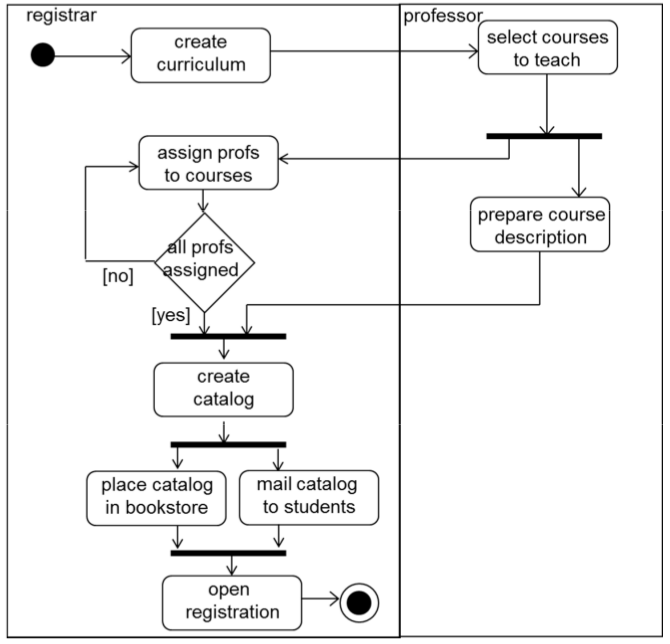
\includegraphics[scale=0.4]{images/activity-diagram.png}
	\item in distributed systems: remote object invocation, middlware (hide the fact, that object is remote, CORBA, COM/DCOM, .net, Java RMi)
	\begin{itemize}
		\item \textbf{CORBA} (Common Object Request Broker Architecture)
		\item object request broker \textsc{Orb} (locate object, activate object, communicate request, return reply) server/servants don't need to be objects (C,Cobol)
		\item \textbf{static} remote interface of CORBA object is known at compile time (code used to generate client stub)
		\item \textbf{dynamic} remote interface not known at compile time
		\item interface definition language \textsc{Idl}: interfaces need to be exactly specified (direct access to variables in remote classes, access only through interface, desired language-independent IDL, that compiles into access methods)
		\item \textsc{Corba Idl} interface specifies names + methods, extended use of C++ syntax
		\begin{description}
			\item[IDL modules] logical grouping of interface/type definitions, defines naming scope
			\item[IDL interface] methods that are available in CORBA objects implementing interface
			\item[IDL methods] specify signatures, parameters are labeled \texttt{in} (from client to server), \texttt{out} (from server to client) and \texttt{inout}, \texttt{oneway} (client will not be blocked on invoking), \texttt{raises} (exceptions)
			\item[IDL attributes] like public fields, may be readonly, get/put methods automatically generated
			\item[IDL interface inheritance] interface may be refinement of other interface
			\item[IDL type names generated by compilter] IDL prefix, type name, prefix number
		\end{description}
		\item CORBA object model (implements IDL interface, has remote object reference, capable of responding to remote invocations)
		\item CORBA has no objects/classes \follows use structs, classes cannot be arguments/results
		\item CORBA can be documented with UML
		\item CORBA architecture
		\begin{description}
			\item[skeltons] generated by IDL compiler, marshaling/unmarshaling of arguments/exceptions
			\item[client stub/proxy] in application language, generated by IDL interface definition, marshaling/unmarshaling of arguments/exceptions
		\end{description}
 	\end{itemize}
 	\item Design-by-Contract\texttrademark \follows Eiffel language
 	\begin{itemize}
 		\item server must \emph{ensure postcondition}, can \emph{assume precondition}
 		\item client must \emph{ensure precondition}, can \emph{assume postcondition}
 		\item UML Object Constraints Language (OCL) \\
 		\begin{tikzpicture}[]

\umlclass{HashTable}{numElements:int}{
put(key,entry;Object) \\
get(key):Object \\
remove(key:Object) \\
containsKey(key:Object):boolean \\
size():int
}

\end{tikzpicture}
 		\begin{description}
 			\item[put] precondition \texttt{!containsKey(key)}, postcondition \texttt{get(key==entry)}
 			\item[get] precondition \texttt{containsKey(key)}, postcondition \texttt{!containsKey(key))}
 			\item[remove] precondition \texttt{containsKey(key)}, postcondition \texttt{!containinsKey(key)}
 		\end{description}
 	\end{itemize}
 	\item \emph{subcontracts} (inheritance), subconstructor may
 	\begin{itemize}
 		\item keep or weaken precondition (more may be let in)
 		\item keep or strengthen postcondition (less may come out)
 	\end{itemize}
 \end{itemize}

\subsection{Data Dictionaries}
\begin{itemize}
	\item low level data decisions \follows late in design process
	\item representation of data structures only known to those with direct data interaction (information hiding)
	\item \textbf{Data Dictionary} list of all names, entities, realtionships, attributes used (name management, avoid duplication, store organisational knowledge)
\end{itemize}

\subsection{Software Architecture and Patterns}
\begin{shaded}
``The \emph{architecture of a software system} defines that system in terms of computational components and interactions among thos components.'' \\
``\dots involves the description of elements from which systems are built, interactions among there elements, patterns that guide their composition, and constraints on these patterns.''
\end{shaded}

\paragraph{Architectural Styles:}
\begin{itemize}
	\item pipe and filter \\ \begin{tikzpicture}[
>=stealth,
node distance=2cm,
arrow/.style={draw,->}
]

\node (empty) at (0,0) {};
\node[draw] (filter) [right of = empty] {filter 1};
\node[draw] (filter2) [right of = filter] {filter 2};
\node[draw] (filter3) [right of = filter2] {filter 3};
\node[draw] (filter4) [above right of = filter2] {filter 4};
\node[draw] (filter5) [below right of = filter2] {filter 5};
\node[draw] (filter6) [right of = filter4] {filter 6};
\node[draw] (filter7) [right of = filter5] {filter 7};
\node[draw] (filter8) [below right of = filter6] {filter 8};
\node (empty2) [right of = filter8] {};

\path[arrow] (empty) -- (filter);
\path[arrow] (filter) -- (filter2);
\path[arrow] (filter2) -- (filter3);
\path[arrow] (filter2) |- (filter4);
\path[arrow] (filter2) |- (filter5);
\path[arrow] (filter4) -- (filter6);
\path[arrow] (filter5) -- (filter7);
\path[arrow] (filter3) -- (filter8);
\path[arrow] (filter6) -| (filter8);
\path[arrow] (filter7) -| (filter8);
\path[arrow] (filter8) -- (empty2);

\end{tikzpicture}
	\item call and return (recommended high fan-in, low fan-out) \\ \begin{tikzpicture}[
>=stealth,
every path/.style={draw,<->},
node distance=1.5cm
]

\node[draw] (root) at (0,0) {M};
	\node[draw] (b) [below of = root] {b};
		\node[draw] (f) [below of = b] {f};
	\node[draw] (a) [left of = b] {a};
		\node[draw] (e) [below of = a] {e};
		\node[draw] (d) [left of = e] {d};
	\node[draw] (c) [right of = b] {c};
		\node[draw] (g) [below of = c] {g};
			 \node[draw] (k) [below of = g] {k};
		\node[draw] (h) [right of = g] {h};
		\node[draw] (i) [right of = h] {i};

\node (fanout) at (1.5,-0.7) {fan-out};
\node (fanin) at (3.8,-4) {fan-in};

\path (root) -- (a);
	\path (a) -- (d);
	\path (a) -- (e);
\path (root) -- (b);
	\path (b) -- (f);
\path (root) -- (c);
	\path (c) -- (g);
	\path (c) -- (h);
	\path (c) -- (i);
		\path (g) -- (k);
		\path (h) -- (k);
		\path (i) -- (k);

\end{tikzpicture}
	\item layers in hirarchical architecture (layer: group of closely related and highly coherent functionalities) \\ \begin{tikzpicture}[
>=stealth,
line/.style={draw},
bigl/.style={draw,line width = 4pt, color=black!50},
root/.style={draw},
func1/.style={draw,fill=yellow!40},
func2/.style={draw,fill=red!40},
func3/.style={draw,fill=blue!40}
]

\node[root] (root) at (0,0) {};

\node[func1] (fu1) at (-3,-1) {};
	\node[func1] (fu12) [below of = fu1] {};
	\node[func1] (fu13) [right of = fu12] {};
		\node[func1] (fu131) [below right of = fu12] {};
		\node[func1] (fu132) [below left of = fu12] {};
	\node[func1] (fu14) [left of = fu12] {};

\node[func2] (fu2) at (0,-1) {};
	\node[func2] (fu22) [below of = fu2] {};
	\node[func2] (fu23) [right of = fu22] {};
	\node[func2] (fu24) [left of = fu22] {};

\node[func3] (fu3) at (3,-1) {};
	\node[func3] (fu31) [below of = fu3] {};

\path[line] (root) -- (fu1);
	\path[line] (fu1) -- (fu13);
	\path[line] (fu1) -- (fu12);
		\path[line] (fu12) -- (fu131);
		\path[line] (fu12) -- (fu132);
	\path[line] (fu1) -- (fu14);

\path[line] (root) -- (fu2);
	\path[line] (fu2) -- (fu22);
	\path[line] (fu2) -- (fu23);
	\path[line] (fu2) -- (fu24);

\path[line] (root) -- (fu3);
	\path[line] (fu3) -- (fu31);

%separators
\path[bigl] (-1.5,0) -- (-1.5,-3);
\path[bigl] (1.5,0) -- (1.5,-3);
%functions
\node (fun1) at (-3,-.5) {function 1};
\node (fun2) at (0,-.5) {function 2};
\node (fun3) at (3,-.5) {function 3};


\end{tikzpicture} \\ \begin{tikzpicture}[
>=stealth,
line/.style={draw},
bigl/.style={draw,line width = 4pt, color=black!50},
root/.style={draw},
func1/.style={draw,fill=yellow!40},
func2/.style={draw,fill=red!40},
]

\node[root] (root) at (0,0) {};

\node[func1] (fu1) at (-3,-1) {};
	\node[func2] (fu12) [below of = fu1] {};
	\node[func2] (fu13) [right of = fu12] {};
	\node[func2] (fu14) [left of = fu12] {};

\node[func1] (fu2) at (0,-1) {};
	\node[func2] (fu22) [below of = fu2] {};
	\node[func2] (fu23) [right of = fu22] {};
	\node[func2] (fu24) [left of = fu22] {};

\node[func1] (fu3) at (3,-1) {};
	\node[func2] (fu31) [below of = fu3] {};

\path[line] (root) -- (fu1);
	\path[line] (fu1) -- (fu13);
	\path[line] (fu1) -- (fu12);
	\path[line] (fu1) -- (fu14);

\path[line] (root) -- (fu2);
	\path[line] (fu2) -- (fu22);
	\path[line] (fu2) -- (fu23);
	\path[line] (fu2) -- (fu24);

\path[line] (root) -- (fu3);
	\path[line] (fu3) -- (fu31);

%separators
\path[bigl] (-4.5,-.5) -- (3.5,-.5);
\path[bigl] (-4.5,-1.5) -- (3.5,-1.5);

%functions
\node (fun1) at (2,0) {decision makers};
\node (fun2) at (0,-2.5) {workers};



\end{tikzpicture}
	\item opaque layering: vm can only callfrom layer below \follows separation of concerns, maintainability, flexibility
	\item transparent layering: vm can call from any layer \follows runtime efficiency (no parameter/message passing, data conversion, format changes)
	\item clients/servers (communication by recipients)
	\begin{description}
		\item[client] process wishing to access data/use resources/perform operations
		\item[server:] process managing data and shared resources
	\end{description}
\end{itemize}
\begin{shaded}
``Each pattern describes a problem which occurs over and over again in our environment, and then describes the core of the solution to that problem, in such a way, that you can use this solution a million times over, without ever doing it the same way twice.'' Christopher Alexander
\end{shaded}
\subsection{Design Patterns}
\begin{itemize}
	\item improved documentation, more abstract level of programming, improved communication
	\item patterns as components, classes
\end{itemize}

\subsubsection{Adapter - Wrapper}
\begin{description}
	\item[Pattern and Name Classification] Adapter Wrapper
	\item[Intent] Anbieten eines alternativen Interfaces für eine Klasse
	\item[Motivation] fremde Klasse mit unpassendem Interface in 
\end{description}

\subsubsection{Brücke}
\begin{description}
	\item[Pattern and Name Classification] Brücke
	\item[Intent] Decouple an abstraction from its implementation so that the two can vary independently.
	\item[Motivation] Eine Brücke kann eine dauerhafte Verbindung zwischen Abstraktion und Implementierung verhindern.
	\item[Applicability] situation in which design pattern can be applied, how to recognize this situations
	\item[Structure] abstract graphical representation
	\item[Participants]
	\item[Collaborations]
	\item[Implementations]
	\item[sample code]
	\item[known uses]
	\item[related patterns]
\end{description}

\subsubsection{Decorator}
\begin{description}
	\item[Pattern and Name Classification] Decorator
	\item[Intent] Fügt individuellen Objekten Zuständigkeiten hinzu, aber nicht der Klasse
	\item[Motivation] Bspw TextArea einen Rahmen und eine ScrollBar hinzufügen
\end{description}

\subsubsection{Facade}
\begin{description}
	\item[Pattern and Name Classification] Facade
	\item[Intent] baut eine Klasse als Fassade vor viele andere Klassen, ermöglicht Methoden, die wieder Methoden in hinteren Klassen aufrufen, vereinfacht Schnittstellen
	\item[Motivation] einfache Klasse für Zugriff von Außen, voller Zugriff auf Methoden des Basissystems
	\item[related patterns] Wrapper, Mediator
\end{description}

\subsubsection{Observer}
\begin{description}
	\item[Pattern and Name Classification] Observer / publish-subscribe
	\item[Intent] Abstrakte Kommunikationsmöglichkeit
	\item[Motivation] Das beobachtete Objekt bietet Anmeldung für Observer an, informiert diese dann über interne Änderungen. Muss Struktur des Observers nicht kennen, meldet einfach jede Änderung weiter \follows Observer muss darauf reagieren können.
\end{description}

\subsubsection{Proxy/Stellvertreter}
\begin{description}
	\item[Pattern and Name Classification]Proxy, Stellvertreter, Surrogat
	\item[Intent] Kontrollierter Zugriff auf ein Objekt mit Hilfe eines vorgelagerten Stellvertreters
	\item[Motivation] Proxy hält eine Referenz auf das reale Objekt, stellt gleich Schnittstelle zur Verfügung
	
\end{description}

\subsubsection{Singelton}
\begin{description}
	\item[Pattern and Name Classification] Singelton
	\item[Intent] Klasse mit genau einer Instanz, normalerweise globaler Zugriff
	\item[Motivation] Klasse hat komplette Zugriffskontrolle, 
	\item[Applicability] Bpsw Druckerbuffer, Filesystem, Window Manager
\end{description}

\subsection{From Design to Code}
\subsubsection{Mapping Design Models to Code}
\begin{description}
	\item[optimization] meet performance requirements (reduce multiplicity of associationsm redundant associations)
	\item[realisation of associations] map asociations to source code
	\item[mapping of contracts to exceptions] raise (and handle) exceptions, when contract broken
	\item[mapping of class models to storage schema] select persistend storage strategy (database, flat files), define relational database schema
	\item[implementation of visibility attributes] private, protected, public
\end{description}

\subsubsection{Implementing Interface Contracts}
\begin{itemize}
	\item most OO languages no built-in support for contracts (except Eiffel)
	\item some OO languages have built-in exception handling support (throw-cath in Java)
	\item check each \emph{precondition} before beginning the method
	\item check each \emph{postcondition} after the method
	\item check \emph{invariants} before and after method
\end{itemize}

\subsubsection{Maping to Relational Databases}
\begin{itemize}
	\item map UML-constructs to tables (not everything can be mapped)
	\item class $\to$ table
	\item class attribute $\to$ column in table
	\item class instance $\to$ row in table
	\item many-to-many associations $\to$ own table
	\item one-to-many $\to$ foreign key
	\item no direct mapping $\to$ do something in sql,\dots
\end{itemize}

\subsection{Documenting Design}
\subsubsection{System Design Document - \textsc{Sdd}}
\begin{enumerate}
	\item Introduction
	\begin{enumerate}
		\item Purpose of system
		\item Design goals
		\item Definitions, acronyms, abbreviations (glossary)
		\item References
		\item Overview
	\end{enumerate}
	\item Current Architecture (only if there is current system available)
	\item Proposed Software Architecture
	\begin{enumerate}
		\item Overview (funtionality of each subsystem)
		\item Subsystem Decomposition (responsibilities of indiv. subsystems, main contrib of SDD)
		\item Hardware/Software mapping
		\item Persistent Data Management (database usage and schemes)
		\item Access control and security (access rights, encryption/key management)
		\item Global software control (initiation of requests, subsystem synchronization, concurrency)
		\item Boundary Conditions (startup, shutdown, error behaviour)
	\end{enumerate}
	\item 
\end{enumerate}

\subsubsection{Object Design Document - \textsc{Odd}}
\begin{enumerate}
	\item Introduction
	\begin{enumerate}
		\item Object design trade-offs (buy vs build, memory vs response time, \dots)
		\item Interface documentation guidelines, coding conventions
		\item Definitions, acronyms, abbreviations
		\item References
	\end{enumerate}
	\item Packages
	\begin{enumerate}
		\item package decomposition and file organistaion of code
	\end{enumerate}
	\item Class Interfaces
	\begin{enumerate}
		\item public interfaces (incl operations, attributes) of each class
		\item dependencies with other classes
	\end{enumerate}
\end{enumerate}
{\tiny part can be done automatically with e.g. JML/Javadoc}

\section{Testing and Software Quality Assurance (\textsc{Sqa})}
\begin{itemize}
	\item about 1 faults per 1000 lines of code
	\item verification and validation techniques (code analysis, review, testing, formal verification), the earlier, the better (cost)
	\begin{description}
		\item[verification] \emph{prove} that a product meets its specification (formal verification, correctness proofs)
		\item[validation] \emph{experiment} with system, to show iot meets requirements (simulating, testing, model cheking)
	\end{description}
	\item code quality assessment (software metrics)
\end{itemize}

\subsection{Software Testing and Strategies}
\subsection{Reviews and Inspections}
\subsubsection{Reviews}
\begin{itemize}
	\item technical meetings (walk-through, inspections)
	\item objectives: software quality assurance, training
	\item non-objectives: progess review, budget, trouble-shooting, reprisals, political intrigue
	\item review leader, standards bearer (SQA), mainenance oracle (devils advocate), recorder, user representative, producer, reviewer
	\item evaluate before review
	\item review product, not producer (ask questions instead of accusing, avoid criticising style \follows technical correctness)
	\item raise issues, don't resolve them
\end{itemize}

\subsubsection{Code walk-through}
\begin{itemize}
	\item ``playing the computer'' \follows ``interpret code''
	\item 3-5 participants
	\item discover, don't fix errors
	\item moderator, secretary, auditors, designer (explain own design)
\end{itemize}

\subsubsection{Code Inspections}
\begin{itemize}
	\item similar to code-walkthrough, different goal: look for commonly made mistakes, no simulation of computers behaviour
	\item unitialized variables, jumps into loops, incompatible assignements, nonterminating loops, array boundaries, storage allocation/deallocation, parameter mismatches
	\item analysis tools can be helpfull
\end{itemize}

\subsection{Test Coverage}
\begin{description}
	\item[white box testing] source is revealed ((code) structural testing)
	\item[black box testing] no source available (test against requirements specification)
	\item[grey box testing] some internal state variables are revealed
\end{description}
\subsubsection{Types of Testing}
\begin{tikzpicture}[%
>=stealth,
node distance=3cm,
on grid,
auto,
multiline/.style={text width=1.8cm,align=center},
square/.style={multiline,draw},
round/.style={multiline,draw,rounded corners=8pt},
dev/.style={fill=blue!20},
cl/.style={fill=red!20},
arrow/.style={draw,thick,->},
bl/.style={draw,line width=3pt}
]

\node[square,dev] (odd) at (0,0) {Object Design Document};
\node[square,dev] (sdd) [right of = odd] {System Design Document};
\node[square,dev] (rad) [right of = sdd] {Requirement Analysis Document};
\node[square,cl] (ce) [right of = rad] {Client Expectation};

\node[round,dev] (ut) [below of = odd] {Unit Testing};
\node[round,dev] (it) [below of = sdd] {Integration Testing};
\node[round,dev] (st) [below of = rad] {System Testing};
\node[round,cl] (at) [below of = ce] {Acceptance Testing};

\node (devel) at (3,-4) {\textcolor{blue!30}{\textbf{Developer}}};
\node (devel) at (9,-4) {\textcolor{red!30}{\textbf{Client}}};

\path[arrow] (odd) -- (ut);
\path[arrow] (sdd) -- (it);
\path[arrow] (rad) -- (st);
\path[arrow] (ce) -- (at);

\path[arrow] (ut) -- (it);
\path[arrow] (it) -- (st);
\path[arrow] (st) -- (at);

\path[bl] (7.5,.8) -- (7.5,-4.5);

\end{tikzpicture}

\begin{description}
	\item[unit/module Testing] check that one module meets design specifications (often during programming)
	\begin{itemize}
		\item to be tested: methods within object, classes with several attributes/methods, components consisting of multiple classes + internal interfaces
		\item it's not testing the system as a whole
		\item complete coverage: testing all operations with all possible combinations of parameters + setting and testing all possible combinations of object attribute values + testing all possible states \follows number blowup
		\item two types of tests:\\
		normal \follows unit does, what it is supposed to do \\
		robustness test \follows when subjected to ``hostile environment'' unit is robust
	\end{itemize}
	\item[integration testing] done during assembly  of complete system, test that modules work together, test that system meets requirements (done by integrators, test specialists)
	\item[system testing] testing the system as a whole
	\item[acceptance testing] test that customer performs when software is delivered (may be fixed in requirement specification or contract)
	\item[regression testing] performed during maintenance/when component has changed (ensure that what worked in the past, will work in the future)
	\item[stress testing] test system under extreme conditions
\end{description}
\subsubsection{formalized testing}
\begin{description}
	\item[$D$:] input domain
	\item[$R$:] arbitrary set, results
	\item[$P$:] patial function, describing programm input/output behaviour: $P:D\to R$
	\item[$OR$:] the output value requirements (from \textsc{Srs})
	\item[testing:]determine where for given $d\in D,P(d)$ meets requirements stated in $OR$, if \follows sucess, else fail
	\item[$d\in D$:] is test case
	\item[$T\subseteq D$:] is test set/suite
	\item[$T$:] is sucessfull, iff all $d\in T$ sucessfull
	\item[$C\subseteq 2^D_f$:]  is selection criterion, $2^D_f$ is set of all finite subsets of $D$
	\item[$T$:] satisfies $C$ iff $T\in C$
	\item[for all $i,k$:] let $T_i,T_k$ satisfy $C$, $C$ is consistent if ($T_i$ is sucessfull iff $T_k$ is sucessfull)
	\item[$C$:] is complete if, when $P$ is incorrect, there is a $T$ satisfying $C$ which is unsucessfull
	\item[if $C$ complete and consistent:] any test $T$ that satisfies $C$ decides $P$'s correctness
\end{description}

\subsubsection{selective testing - how many paths to test?}
\begin{description}
	\item[Statement Coverage] select $T$ s.t. by executing $P(d)$ for every $d\in T$, \textbf{each statement is at least executed once} {\tiny statement \follows square}
	\item[edge coverage] select $T$ s.t. \textbf{each edge in control flow graph is traversed at least once}
	\item[condition coverage] select $T$ s.t. \textbf{edge coverage is satisfied and all possible values for consituent proposition inside conditions are exercised at least once} {\tiny each check must be executed}
	\item[multiple condition coverage] each boolean combination of the consitutent predicates of every condition needs to be exercised at least once {\tiny each combination (of sucess/failure) at least once}
	\item[path coverage] select $T$ s.t. all paths from an inital ndoe to a final node in the control flow graph are traversed at least once
\end{description}

\subsubsection{Basis Path Testing}
\begin{itemize}
	\item assess how many tests are needed to achieve statement \& path coverage (prog is single entry, single exit, control flow graph available, all decisions binary)
	\item calculate cyclomatic complexity $V(G)$
	\begin{itemize}
		\item $V(G)=$ \# of simple decissions $+1$
		\item $V(G)=$ \# of enclosed areas $+1$
	\end{itemize}
	\item loop testing ($n$ is number of allowable passes)
	\begin{enumerate}
		\item skip the loop
		\item one pass
		\item two passes
		\item $m$ passes through loop, $m<n$
		\item $(n-1), n, (n+1)$ passes through the loop
	\end{enumerate}
\end{itemize}

\subsubsection{testing based on contracts}
\begin{itemize}
	\item possible test selection criteria
	\begin{itemize}
		\item input conform with the precondition
		\item inputs with a violated precondition
		\item inputs where key element is of correct type
		\item inputs where key element is of wrong type
	\end{itemize}
\end{itemize}

\subsubsection{Acceptance Testing}
\begin{itemize}
	\item demonstrate system is ready for operational use
	\item choice of tests by client, is conducted by client
	\item may be part of contract
	\item alpha test: tests in devs environment, beta test: tests in clients environment
\end{itemize}

\subsubsection{integration testing}
\begin{itemize}
	\item driver: component that calls the \texttt{testedUnit}, controls test cases
	\item stub: component that the \texttt{testedUnit} depends on (``fake'')
	\item big bang - just put together and see, if it works
	\item top-down - tests the top layer first, then downward \follows stubs are needed, test can be designed by the functionality of system
	\item bottom-up - subsystem in lowest layer testet first \follows drivers are needed (test ui (most important part) last)
	\item sandwich - combination of bottom-up and top-down, converges at target layer \follows does not test individual layers thouroghly
	\item modified sandwich - combination of all other tests
\end{itemize}

\subsubsection{Testplan}
\begin{enumerate}
	\item Einführung (Beschreibung der Testobjekte)
	\item Bezug zu anderen Dokumenten (RAD, SDD, \dots)
	\item Systemübersicht (strukturelle Aspekte des Tests, Übersicht auf die zu testenden Objekte)
	\item Features zum Testen und Nicht-Testen (funktionale Aspekte, Beschreibung der zu testenden Features)
	\item Pass/Fail-Kriterien
	\item Approach (Herangehensweise an Testprozess, Grund für Wahl einer Teststrategie)
	\item Suspension \& Resumption (Kriterien zum Unterbrechen eines Tests, Spezifizierung der Testabläufe nach Wiederaufnahme)
	\item Testmaterial (benötigte Resourcen)
	\item Testfälle (Test Case Specification, Test Incident Report)
	\item Testing Schedule (Verantwortlichkeiten, Personalbedarf, Risiken, Kosten, Ablaufplan)
\end{enumerate}
\paragraph{Test Case Specification}
\begin{enumerate}
	\item Testfallbezeichner (Name)
	\item Test items (Komponenten und Features)
	\item Eingabespezifikationen
	\item Ausgabespezifikationen
	\item Umgebungsanforderungen (HW/SW)
	\item Besondere prozedurale Anforderungen (Zeitlimits, \dots)
	\item Abhängigkeit zwischen Fällen
\end{enumerate}

\subsection{Software Metrics}
\subsubsection{McCabe's Cyclomatic Complexity}
\begin{itemize}
	\item determine control flow graph
	\item Cyclomatic Complexity $C=e-n+2p$ ($e$ - edges, $n$ - nodes, $p$ - number of connected components (1 for totally connected)) \\
	\item $C$ determines number of paths
	\item no GoTos, single entry/single exit \follows $C-1$ number of decission nodes
	\item $3\leq C\leq 7$ \follows good values, $C=10$ \follows maximum
\end{itemize}

\subsubsection{Software Product Metrics}
\begin{description}
	\item[fan-in/fan-out] number of functions or methods, that call other functions or methods (X). Fan-out is the number of functions, thar are called by X. High Fan-in shows tight coupling (changes to X not good), high Fan-out suggests high complexity
	\item[length of code] larger programm \follows more errors
	\item[Cyclomatic Complexity]
	\item[Length of Identifiers] longer identifiers are simpler to understand
	\item[depth of conditional nesting] deep nesting is hard to understand
	\item[fog index] average length of words and sentences in documents, higher fog is harder to understand
 \end{description}

\subsubsection{Object-Oriented Software Metrics}
\begin{description}
	\item[depth of inheritance tree] deeper inheritance tree \follows more complex design
	\item[Method fan-in/fan-out] distringuish between internal (good) and external (bad) methods, see above
	\item[weighted methods per class] number of methods in a class weighted by its complexity \follows high value is bad
	\item[number of overriding operations] high value indicates, superclass not good model for subclass
\end{description}

\subsection{Formal verification}
das lass ich mal weg, das seh ich als nicht wichtig an

\end{document}
